\chapter{Tests du prototype}
\label{ch:test}

Les tests sont une partie importante de tout projet.
Cependant, pour des raisons éthiques (voir chapitre \ref{ch:etudemoralite}), légales (voir chapitre \ref{ch:etudelegislation}) et logistiques (à cause des mesures de confinement depuis mars 2020)
il a été impossible de tester les divers aspects du prototype en conditions réelles.

\section{Tests de l'algorithme PP2I}
La partie la plus critique à tester est celle concernant l'algorithme PP2I. 
En effet, c'est le point pouvant causer le plus d'erreurs lors du processus.
C'est pourquoi un module de \textbf{simulation} a été développé. 

\subsection{Explication de la simulation}
La simulation est exécutée à la création de la base de donnée.
Selon les paramètres passés au script de création, un certain nombre d'identités vont être générées. 
À chaque identité est associée une adresse MAC connue. 
Une boucle d'événement est exécutée à chaque unité de temps de la simulation (une minute)   
Durant cette boucle, chaque identité à une certaine probabilité d'émettre une probe request contenant son adresse MAC ou 
d'être "pris en photo". Lorsque la simulation est terminée, toutes ces données sont analysées et la correspondance des couples Adresse MAC - Identité est faite. 

Comme nous connaissant la véritable adresse de chaque identité, nous pouvons calculer un taux de réussite correspondant au nombre d'identités ayant reçu la bonne adresse MAC par rapport au nombre d'identités total.

\subsection{Exemple de graphique résultant de la simulation}
Les informations clés de la simulation sont compilées dans un graphique au format de la figure \ref{fig:simulation-result-example} 
\begin{figure}[H]
	\centering
	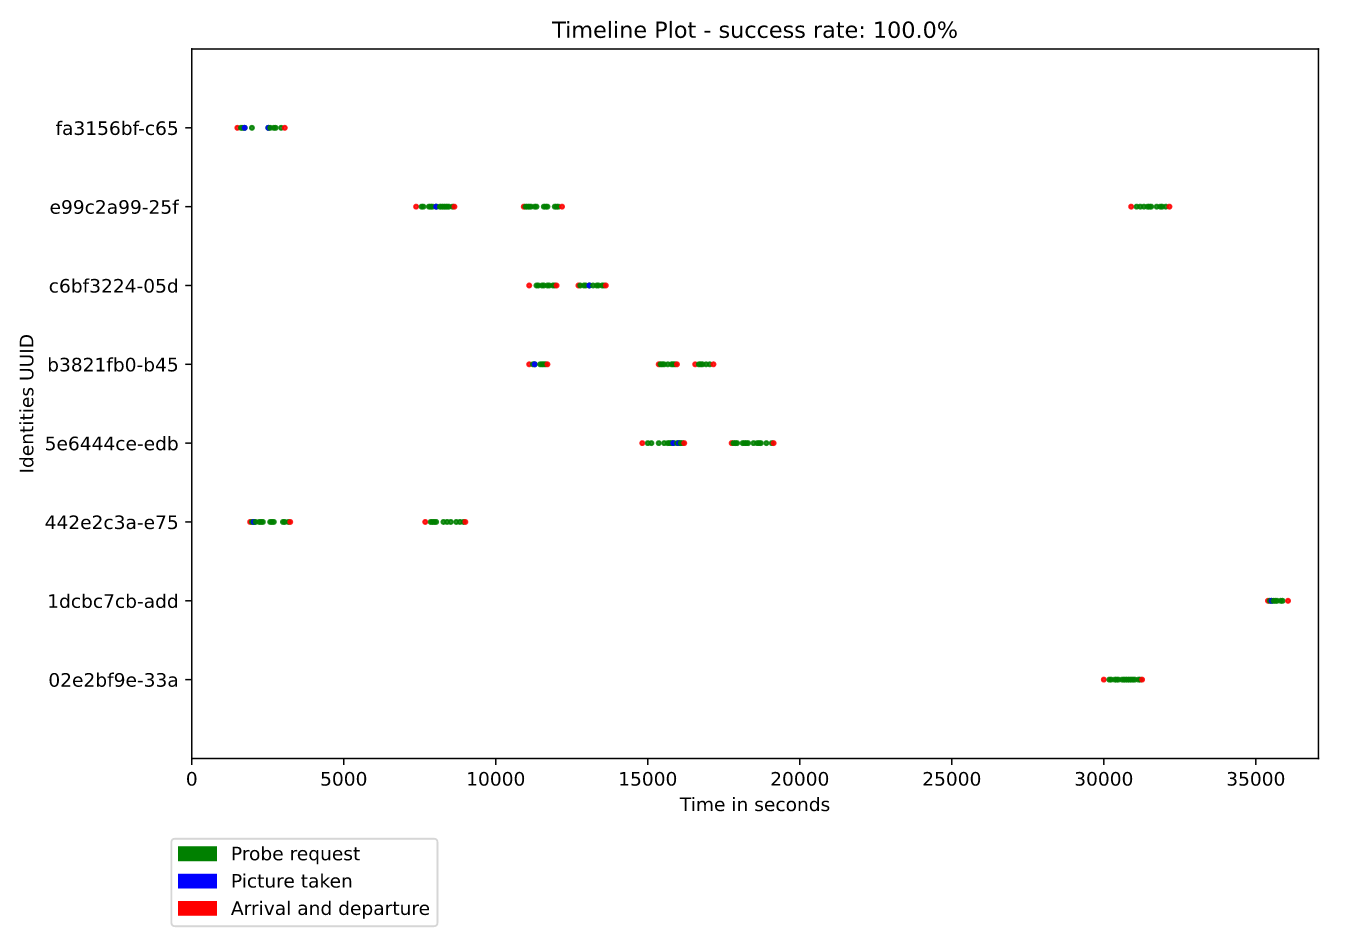
\includegraphics[width=12cm]{images/tests/exemple-graph.png}
	\caption{Exemple de résultat de la simulation}
	\label{fig:simulation-result-example}
\end{figure}

Voici les éléments importants du graphique et leur signification:
\begin{itemize}
    \item Le titre du graphique indique le taux de réussite
    \item L'axe des abcisses indique le déroulement du temps lors de la simulation
    \item L'axe des ordonnées indique un identifiant unique par identité (UUID). Un UUID en rouge indique que l'algorithme PP2I n'a pas assigné la bonne adresse MAC à cette identité 
    \item Chaque point sur la frise chronologique indique un événement dont la couleur indique la nature
\end{itemize}

\subsection{Choix d'implémentation}
Pour simuler au mieux les tests qui auraient pu être effectués en condition réelle, les décisions suivantes ont été prises:

Chaque visite d'une personne est modélisée selon une distribution normale (comme le temps de visite moyen dans un centre commercial par exemple) selon la fonction
\[f(x)=\frac{1}{\sqrt{2\pi \sigma^2}} e^{-\frac{1}{2\sigma^2}(x-\mu)^2}\]

\begin{figure}[H]
\begin{tikzpicture}
\begin{axis}[every axis plot post/.append style={
  mark=none,domain=0:40,samples=50,smooth},
    % All plots: from -2:2, 50 samples, smooth, no marks
  axis x line*=bottom, % no box around the plot, only x and y axis
  axis y line*=left, % the * suppresses the arrow tips
  enlargelimits=upper,
  legend style={at={(0,-0.15)},anchor=west}] % extend the axes a bit to the right and top
  \addplot {gauss(20,5)};
  
  \addlegendentry{$\sigma$ = 5 et $\mu$ = 20}
\end{axis}
\end{tikzpicture}
\caption{Distrubtion continue du temps de visite dans la simulation}
\end{figure}

Une personne peut faire entre une et quatre visite par simulation.
La distribution discrète de probabilité diminue exponentiellement, puisqu'il est peu probable que quelqu'un décide de revenir:

\tikzset{
  % define the bar graph element
  bar/.pic={
    \fill (-.1,0) rectangle (.1,#1) (0,#1) node[above,scale=1/2]{$#1$};
  }
}
\begin{figure}[H]
  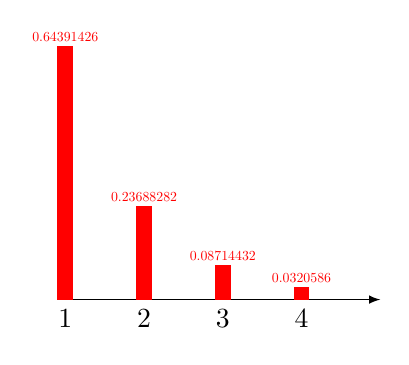
\begin{tikzpicture}[y=5cm]
    \draw
      % the main axis
      (1,0) edge[-latex] (5,0)
      % draw the distribution and label it
      foreach[count=\i from 1] ~ in {0.64391426, 0.23688282, 0.08714432, 0.0320586}{
        (\i,0) pic[red]{bar=~} node[below]{$\i$}
      };
  \end{tikzpicture}
  \caption{Distrubtion discrète du nombre de visite par visiteur lors de la simulation}
\end{figure}

La probabilité à chaque minute de sniffer une probe request est de 60\%, et de 5\% pour les photos. (Il est bien plus difficile de prendre une photo du visage que de 
capter une paquet à distance.) Il est à noté qu'il s'agit d'une estimation.

\section{Protocole de test}
Deux paramètres vont grandement influencer le résultat et vont guider les tests:
\begin{enumerate}
    \item La durée de la simulation
    \item Le nombre d'identités pouvant se présenter
\end{enumerate}

Six tests vont être effectués, avec un exemple commenté pour chaque catégorie: 
\begin{enumerate}
    \item Fréquentation faible pour une simulation de durée courte
    \item Fréquentation moyenne pour une simulation de durée courte
    \item Fréquentation élevée pour une simulation de durée courte
    \item Fréquentation faible pour une simulation de durée longue
    \item Fréquentation moyenne pour une simulation de durée longue
    \item Fréquentation élevée pour une simulation de durée longue
\end{enumerate}

Chaque test va être exécuté plusieurs fois, et les graphiques résultants seront exportés. 
\section{Tests}
\begin{itemize}
    \item La fréquentation faible est représentée par 10 identités.
    \item La fréquentation moyenne est représentée par 50 identités.
    \item La fréquentation élevée est représentée par 150 identités.
\end{itemize}
\begin{itemize}
    \item Une durée courte est représentée par 5h.
    \item Une durée longue est représentée par 30h.
\end{itemize}


\subsection{Fréquentation faible pour une simulation de durée courte}
Pour ce test, la moyenne est de 83.85\% et la médiane est de 81.25\%.
La durée courte engendre des visites simultanées, ce qui rend impossible l'assignation de certaines adresse, mais
le nombre limité de personne mitige ce phénomème. 

Sur la figure \ref{fig:simulation-short-low} on peut toutefois voir que la première identité a reçu la mauvaise adresse.
C'est sûrement car ses événements sont presque un sous-ensemble de ceux émis par la troisième identité.

On peut également observer qu'il n'y a que 6 identités sur cette expérience. C'est car il y a 4 identités
qui n'ont pas émis de photos, et qui ne sont donc pas considérés par l'algorithme.

\begin{figure}[H]
	\centering
	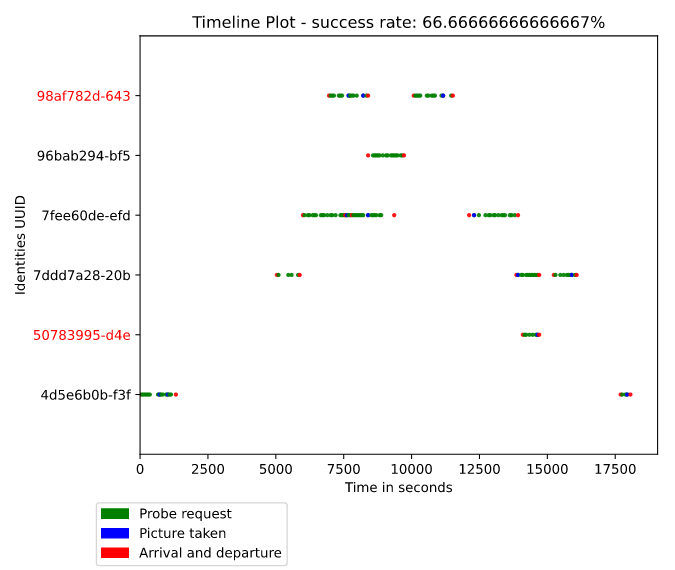
\includegraphics[width=12cm]{images/tests/exemple_courte_faible.png}
	\caption{Exemple de résultat de la simulation à durée courte et fréquentation faible}
	\label{fig:simulation-short-low}
\end{figure}

\subsection{Fréquentation moyenne pour une simulation de durée courte}
Pour ce test, la moyenne est de 61.25\% et la médiane est de 60.52\%.

Les résultats diminuent par rapport au test précédent car le risque de "collisions" augmente.

\subsection{Fréquentation élevée pour une simulation de durée courte}
Pour ce test, la moyenne est de 41.18\% et la médiane est de 41.88\%.

Ce cas de test est le pire de notre matrice. Il devient alors nécessaire d'attendre de nouvelles visites des identités
repérées pour pouvoir être convaincu de résultat de l'algorithme. Heureusement, le but du dispositif WiFace est d'être placé sur le long terme, rendant envisageable la capture des
visites suivantes.

\subsection{Fréquentation faible pour une simulation de durée longue}
Pour ce test, la moyenne est de 96.25\% et la médiane est de 100\%.

Les événements "se diluent" dans une grande période, ce qui rend très fiable l'algorithme. 
Cependant, certains exécutions n'atteigne pas la perfection. On pourrait par exemple considérer le cas d'une 
visite de groupe. Chaque membre va potentiellement émettre des probes requests simultanément, rendant inefficace la détection.
Une telle occurence pourrait être imagée par les deux identités en rouge sur la figure \ref{fig:simulation-long-low}
\clearpage
\newpage
\thispagestyle{empty}
\begin{landscape}
    \centering
\thispagestyle{empty}
\begin{figure}[h]
	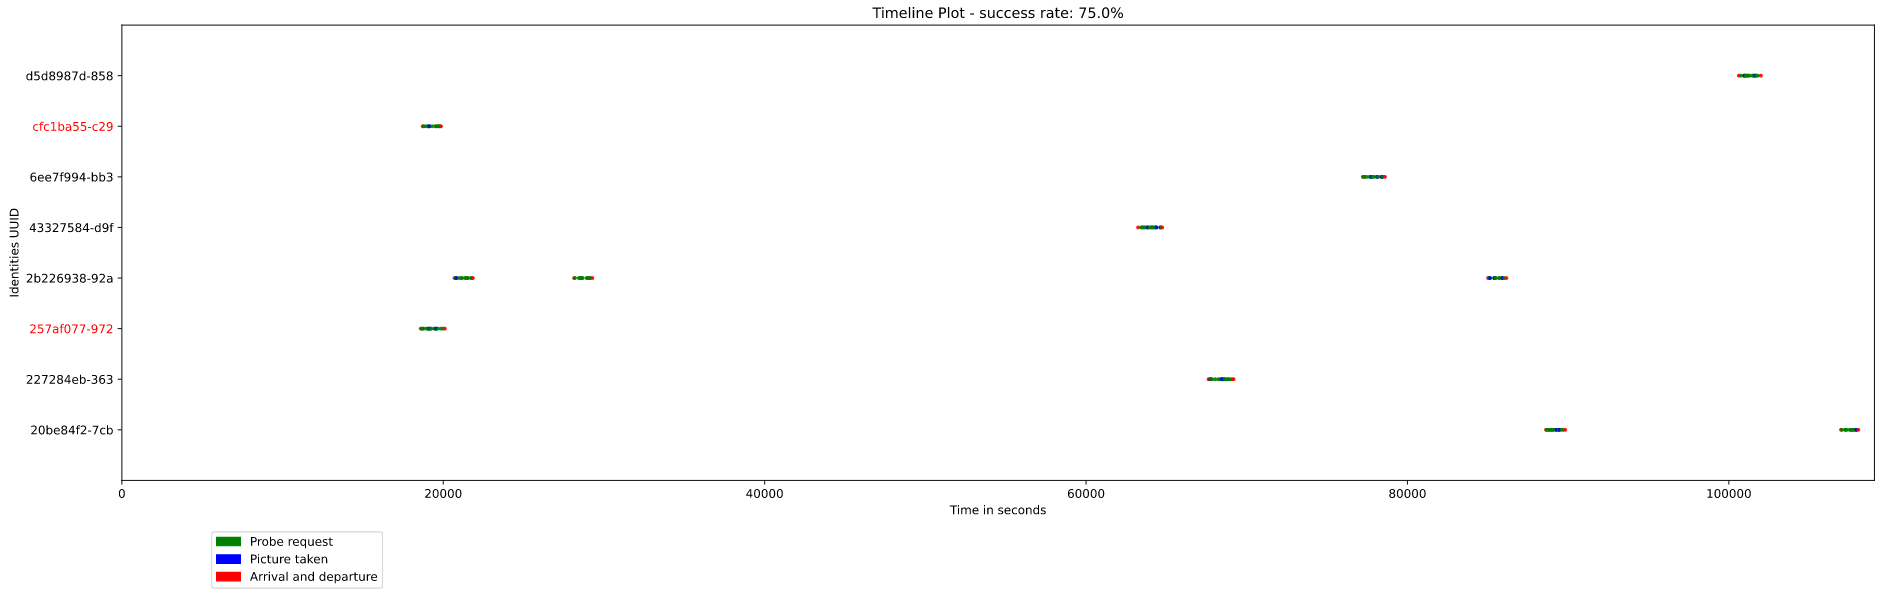
\includegraphics[width=\linewidth]{images/tests/exemple_longue_faible.png}
	\caption{Exemple de résultat de la simulation à durée courte et fréquentation faible}
	\label{fig:simulation-long-low}
\end{figure}
\end{landscape}

\subsection{Fréquentation moyenne pour une simulation de durée longue}
Pour ce test, la moyenne est de 84.43\% et la médiane est de 86.48\%.
Les résultats sont satisfaisants et bien meilleurs qu'en durée courte.

\subsection{Fréquentation élevée pour une simulation de durée longue}
Pour ce test, la moyenne est de 74.58\% et la médiane est de 75\%.

Il s'agit du cas d'utilisation du système le plus probable. 
Posé sur le long terme (bien plus que 30h, mais cette durée a été choisie pour faciliter la simulation), beaucoup de gens fréquenterait l'endroit d'action du dispositif.

\subsection{Synthèse des résultats}

Le tableau \ref{tab:synthese_pp2i} résume les résultats obtenus lors des tests.

\begin{table}[H]
    \begin{tabular}{lllll}
                          & \multicolumn{2}{c}{Durée courte} & \multicolumn{2}{c}{Durée longue} \\
                          & Moyenne         & Médiane        & Moyenne        & Médiane         \\
    Fréquentation faible  & 83.85\%         & 81.25\%        & 96.25\%        & 100.00\%        \\
    Fréquentation moyenne & 61.25\%         & 60.52\%        & 84.43\%        & 86.48\%         \\
    Fréquentation forte   & 41.18\%         & 41.88\%        & 74.58\%        & 75.00\%        
    \end{tabular}
\caption{Synthèse des résultats des tests PP2I}
\label{tab:synthese_pp2i}
\end{table}

\begin{figure}[H]
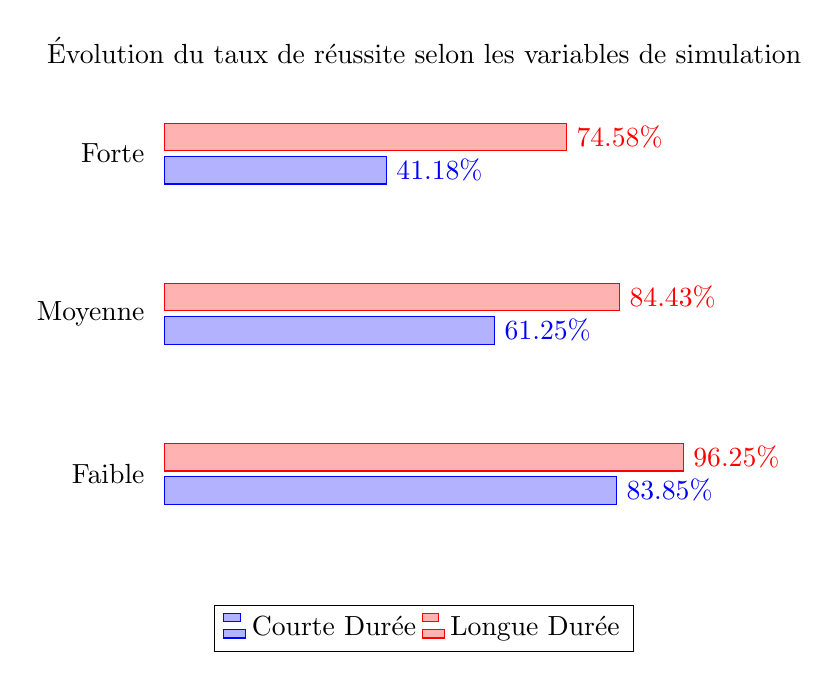
\begin{tikzpicture}
  \begin{axis}
  [
    title    = Évolution du taux de réussite selon les variables de 
              simulation,
    xbar,
    y axis line style = { opacity = 0 },
    axis x line       = none,
    tickwidth         = 0pt,
    ytick distance=1,
    enlarge y limits  = 0.2,
    enlarge x limits  = 0.02,
    nodes near coords={\pgfmathprintnumber\pgfplotspointmeta\%},
    symbolic y coords = {Faible, Moyenne, Forte},
    xmin=0,
    legend style={at={(0.5,-0.15)},
		anchor=north,legend columns=-1},
  ]
  \addplot coordinates { (83.85,Faible) (61.25,Moyenne)
  (41.18,Forte)};
  \addplot coordinates { (96.25,Faible) (84.43,Moyenne) (74.58,Forte)};
  \legend{Courte Durée, Longue Durée}
  \end{axis}
  \end{tikzpicture}
  \caption{Évolution du taux de réussite selon les variables de simulation}
\end{figure}
  
Pour conclure, nous pouvons affirmer que les résultats sont satisfaisants et démontre une valeur ajoutée de l'algorithme PP2I. 
Il existe toutefois divers problèmes qui n'ont pas pu être résolu et qui baisse les performances. Parmi ces problèmes, il y a notamment:
\begin{itemize}
    \item Les visites de groupes qui rendent indiscernables les membres individuellement (sauf si une nouvelle visite séparée du groupe se produit)
    \item Lorsque la période d'activité est trop saturée (peu de temps ou grande fréquentation)
    \item Il est difficile de prendre des photographies (ce qui a été simulé avec un petit pourcentage), ce qui amène parfois à des nuages de points représentant des probe requests, sans image, faussant ainsi le calcul du score.
    \item Les adresses MAC aléatoires ne sont implémentées dans la simulation mais aurait comme conséquence l'ajout de bruit dans la détection 
\end{itemize}





